\documentclass{beamer}
%
% Choose how your presentation looks.
%
% For more themes, color themes and font themes, see:
% http://deic.uab.es/~iblanes/beamer_gallery/index_by_theme.html
%
\mode<presentation>
{
  \usetheme{metropolis}      % or try Darmstadt, Madrid, Warsaw, ...
  \usecolortheme{default} % or try albatross, beaver, crane, ...
  \usefonttheme{default}  % or try serif, structurebold, ...
  \setbeamertemplate{navigation symbols}{}
  \setbeamertemplate{caption}[numbered]
}

\usepackage[frenchb]{babel}
\usepackage[utf8x]{inputenc}
\usepackage[T1]{fontenc}
\usepackage{extramarks} % Required for headers and footers
\usepackage{listings} % Required for insertion of code
\usepackage{amsmath}
\usepackage{hyperref}
\usepackage{textcomp}
\usepackage{stmaryrd}
\usepackage{amsfonts}
\usepackage{framed}

\title[Parallélisation de l'algorithme de Jacobi]{Projet : Parallélisation de la Méthode de Jacobi pour la résolution de systèmes linéaires}
\author{Plessia Stanislas}
\institute{}
\date{Mars 2018}

\begin{document}

\begin{frame}
  \titlepage
\end{frame}

\section{Méthode de Jacobi}

\begin{frame}{Définition du problème}
  Soit :
  \begin{itemize}
   \item $n \in \mathbb{N}$ 
   \item $A = (a_{i,j})_{i,j \in \llbracket 1,n \rrbracket^2}$ matrice carrée de taille $n$
   \item $b = (b_i)_{i \in \llbracket 1,n \rrbracket}$ vecteur de taille $n$.
  \end{itemize}

  On cherche alors le vecteur $x = (x_i)_{i \in \llbracket 1,n \rrbracket}$ tel que :

  \begin{equation} 
      \label{eq:probleme}
      Ax = b
  \end{equation}
\end{frame}

\begin{frame}{Résolution: Decomposition de $A$}
  On décompose $A$ en deux matrices :
  \[
  A =
    \begin{pmatrix}
    a_{1,1} & 0 & \cdots & 0 \\
    0 & a_{2,2} & \cdots & 0 \\
    \vdots  & \vdots  & \ddots & \vdots  \\
    0 & 0 & \cdots & a_{n,n}
   \end{pmatrix}
   +
    \begin{pmatrix}
    0 & a_{1,2} & \cdots & a_{1,n} \\
    a_{2,1} & 0 & \cdots & a_{2,n} \\
    \vdots  & \vdots  & \ddots & \vdots  \\
    a_{n,1} & a_{n,2} & \cdots & 0
   \end{pmatrix}
  \]

  Notons $D$ la matrice diagonale et $R$ le reste.
  Comme on suppose les coefficiens diagonaux non nuls, $D$ est trivialement inversible et on peut transformer l'équation \eqref{eq:probleme} :
  \[
    x = D^{-1}(b - Rx)
  \]
\end{frame}

\begin{frame}{Résolution: Solution Itérative}

  Un solution itérative peut \^etre construite de la manière suivante :
  \[
      \left\{
      \begin{array}{l}
          x^{(0)} = \vec{0}\\
          x^{(k+1)} = D^{-1}( b - Rx^{(k)})
      \end{array}
      \right.
  \]
  D'après le théorème du point fixe, on peut montrer qu'on a alors :
  \[
  \lim_{k \to \infty}x^{(k)} = x \Leftrightarrow \rho(-D^{-1}R) < 1
  \]
  On obtient alors la formule de récurrence sur les coefficients :
  \begin{align} \label{eq:recu}
      \forall k \in \mathbb{N}, \forall i \in \llbracket 1,n \rrbracket, 
      \qquad x_{i}^{(k+1)} = \dfrac{1}{a_{i,i}}(b_i - \sum_{i \neq j}a_{i,j} x^{(k)}_j)
  \end{align}

\end{frame}

\begin{frame}{Résolution: Condition suffisante de convergence}
  Une condition suffisante pour assurer la convergence de la méthode de Jacobi est la suivante:\\

  Soit $\lambda$ valeur propre de $C$ et $y_{\lambda}$le vecteur propre associé, on a :
  \begin{align*}
    |\lambda|\cdot||y_{\lambda}||_{\infty} &= |\dfrac{1}{a_{i,i}}| \cdot |\sum_{j \neq i}a_{i,j}y_{\lambda{j}}|\\
    &\leq |\dfrac{1}{a_{i,i}}| \cdot \sum_{j \neq i}|a_{i,j}| \cdot ||y_\lambda||_{\infty}
  \end{align*} 

  Donc on a $\forall (i,j) \in \llbracket 1,n \rrbracket^2 \quad |a_{i,i}| > \sum_{i \neq j}|a_{i,j}| \implies \rho(C) < 1$,\\
  ie $C$ est a diagonale strictement dominante.
\end{frame}

\section{Implémentation de la Méthode}

\begin{frame}{Structures de données et Librairies}
  \begin{itemize}
    \item Structures de données dynamiques (Matrix, Vector)
    \item Implémentées dans des librairies séparées
    \item Set de fonctions utilitaires pour chaque structures :
    \begin{itemize}
      \item \texttt{build\_structure} 
      \item \texttt{display\_structure}
      \item \texttt{randomize\_structure}
      \item \texttt{free\_structure}
      \item \texttt{read\_structure\_from\_file}
    \end{itemize}
  \end{itemize}
\end{frame}

\begin{frame}[fragile]{Structures de données et Librairies}
  Les structures de données sont implémentées par des types complexes contenant des données de taille (en entier non signés) et un tableau contenant les données de calcul.

  Par exemple pour la structure matrice :
  \begin{lstlisting}[language=C]
  typedef struct Matrix{
      unsigned int col;
      unsigned int rows;
      double **matrix; 
  }Matrix;
  \end{lstlisting}
\end{frame}

\begin{frame}{Programme principal}
Pour paralléliser le programme, nous devons distribuer les données dans les différent processeurs :

Soit \(n\) la taille du problème et \(p\) le nombre processeurs.
Pour le processus \(i\), en notant \(q = \lfloor \frac{n}{p} \rfloor\) et \(r = \text{mod}(n,p)\) :
\begin{itemize}
    \item Nombre de lignes \(N\):  \(q+1\) si \(i<r\), \(q\) sinon;
    \item Première ligne \(F\):  \((q+1)i\) si \(i<r\), \(q\cdot i\) sinon;
\end{itemize}
\end{frame}

\begin{frame}{Programme principal}
  \begin{itemize}
    \item L'équation \eqref{eq:recu} n'a pas de dépendance verticale sur la matrice, elle est donc facilement parallélisable
    \item Les processeurs auront 2 variables locales : \texttt{local\_result} de taille \(N\) et \texttt{global\_result} de taille \(n\) contenant $x^{(k)}$
    \item Au début d'une itération, chaque processeur communique son \texttt{local\_result} pour remplir les \texttt{global\_result} nécessitant d'\^etre complet pour l'itération suivante.
    \item On applique ensuite la formule de récurrence pour mettre à jour \texttt{local\_result}
  \end{itemize}
\end{frame}

\begin{frame}{Convergence}
  Soit $\epsilon^{(k)} = ||x - x^{(k)}||_{\infty}$ et $e^{(k)} = ||x^{(k+1)} - x^{(k)}||_{\infty}$

  On a : 
  \begin{align*}
      e^{(k)} &= ||x^{(k+1)} - x^{(k)}||_{\infty}\\
      &= ||Cx^{(k)} + d - x^{(k)}||_{\infty}\\
      &= ||Cx^{(k)} + x - Cx - x^{(k)}||_{\infty}\\
      &= ||(-C + I)(x - x^{(k)})||_{\infty}
  \end{align*}

  Finalement : $e^{(k)} = ||I - C||_{\infty}\epsilon^{(k)} \leq \epsilon^{(k)} + ||C||_{\infty}\epsilon^{(k)} \leq 2\epsilon^{(k)}$\\
  On peut donc utiliser $e^{(k)}$ comme critère d'arr\^et pour l'algorithme.
\end{frame}

\begin{frame}{Arr\^et}
  Pour décider de l'arr\^et du programme, nous avons une condition pour chaque processeur qui une fois rempli renvoi un booléen au processeur root:
  \begin{itemize}
    \item chaque processeur a un tableau de booléens \texttt{continue\_iterate} de taille \(N\)
    \item quand une ligne a atteind la convergence ($e^{(k)}_{i} = x^{(k+1)}[i] - x^{(k)}[i] \leq 1.10^{-6}$) l'indice $i$ du tableau est inversée (true $\rightarrow$ false)
    \item On affecte la variable \texttt{local\_continue\_to\_process $|=$ continue\_iterate[i] $\forall i$}
    \item run $|=$ local\_continue\_to\_process $\forall$ processeur
  \end{itemize}

\end{frame}

\section{Résultats}

\begin{frame}{Performances}
  \begin{figure}
    \centering
    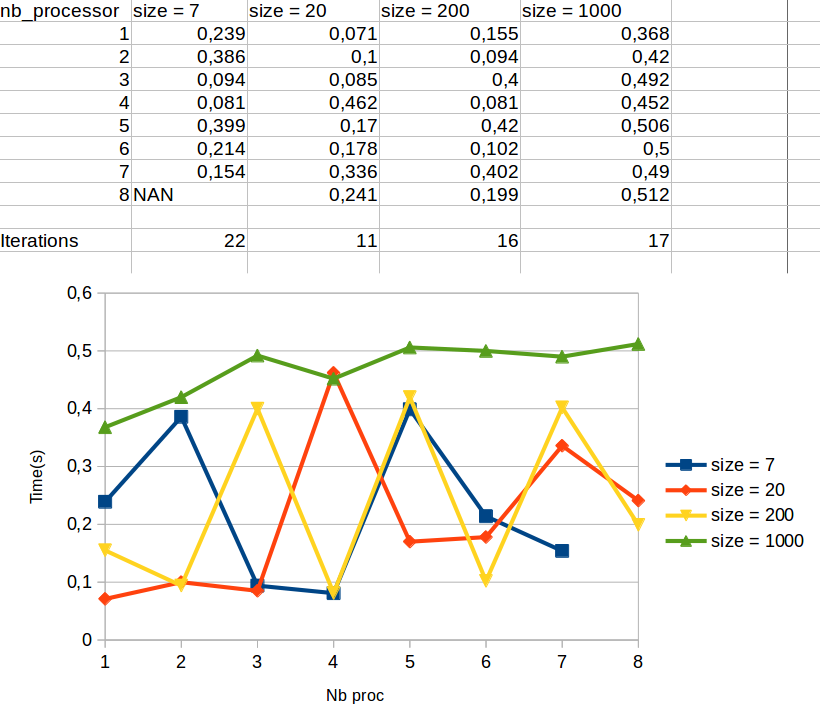
\includegraphics[width=200pt]{perf.png}
    \caption{Tableau des performances du programme en fonction du nombre de processeur et des dimensions du problème}
  \end{figure}
\end{frame}

\begin{frame}{Limites et Améliorations}
  \begin{itemize}
    \item Données essayées non représentatives : Matrices de tailles supérieur à 7 générées par un script qui génère des matrice peu denses
    \item Le programme semble tourner en moyenne aussi rapidement peu importe la taille du problème
    \item Pas d'analyse de l'impact mémoire
    \item Désynchronisations possibles, ne semblent pas arriver sur des petites dimensions, non vérifé sur des grandes dimensions
  \end{itemize}
\end{frame}

\end{document}